%%%%%%%%%%%%%%%%%%%%%%%%%%%%%%%%%%%%%%%%%%%%%%%%%%%%%%%%%%%%%%%%%%%%%%%%%%%%%%%%
% TUM-Vorlage: Präsentation - Beispiele
%%%%%%%%%%%%%%%%%%%%%%%%%%%%%%%%%%%%%%%%%%%%%%%%%%%%%%%%%%%%%%%%%%%%%%%%%%%%%%%%


\begin{frame}[fragile]
\frametitle{Example of new input file}

 \begin{Verbatim}
#Random comments
# xyz-coord      velocity        mass       shape       dimensions      distance  
2
0.0 0.0 0.0      0.0 0.0 0.0     1.0
7.0 7.0 7.0      1.0 1.0 1.0     2.0e-8     CuboiD      4	5	6         3.0
# epsilon    sigma
0.1         0.2
 \end{Verbatim}

\vspace{-0.5cm}
\large
Structure:
\vspace{-0.7cm}
\begin{itemize}
	\item<1-> Comments
	\item<1-> Number of bodies
	\item<2-> Bodies (with Shape, Dimensions and distance as optional)
	\item<3-> Comments
	\item<4- > Definition of epsilon and sigma (optional)
\end{itemize}

\end{frame}

\begin{frame}
	\frametitle{CI/CD}
	\large
	\begin{itemize}
		\item<1-> Protection of master branch
		\item<2-> Deployment of CI/CD pipeline for \textit{all} branches 
	\end{itemize}

\end{frame}

\begin{frame}
	\frametitle{CI/CD}
	\large
	\begin{itemize}
		\item Protection of master branch
		\item Deployment of CI/CD pipeline for \textit{all} branches 
	\end{itemize}
	\Large
	The pipeline consist of:
	\large
	\begin{itemize}
		\item<1-> library installment
		\item<2-> build process
		\item<3-> sanitizers
		\item<4-> custom tests
	\end{itemize}
\end{frame}

\begin{frame}
	\frametitle{IO}
	\begin{figure}
		\centering
		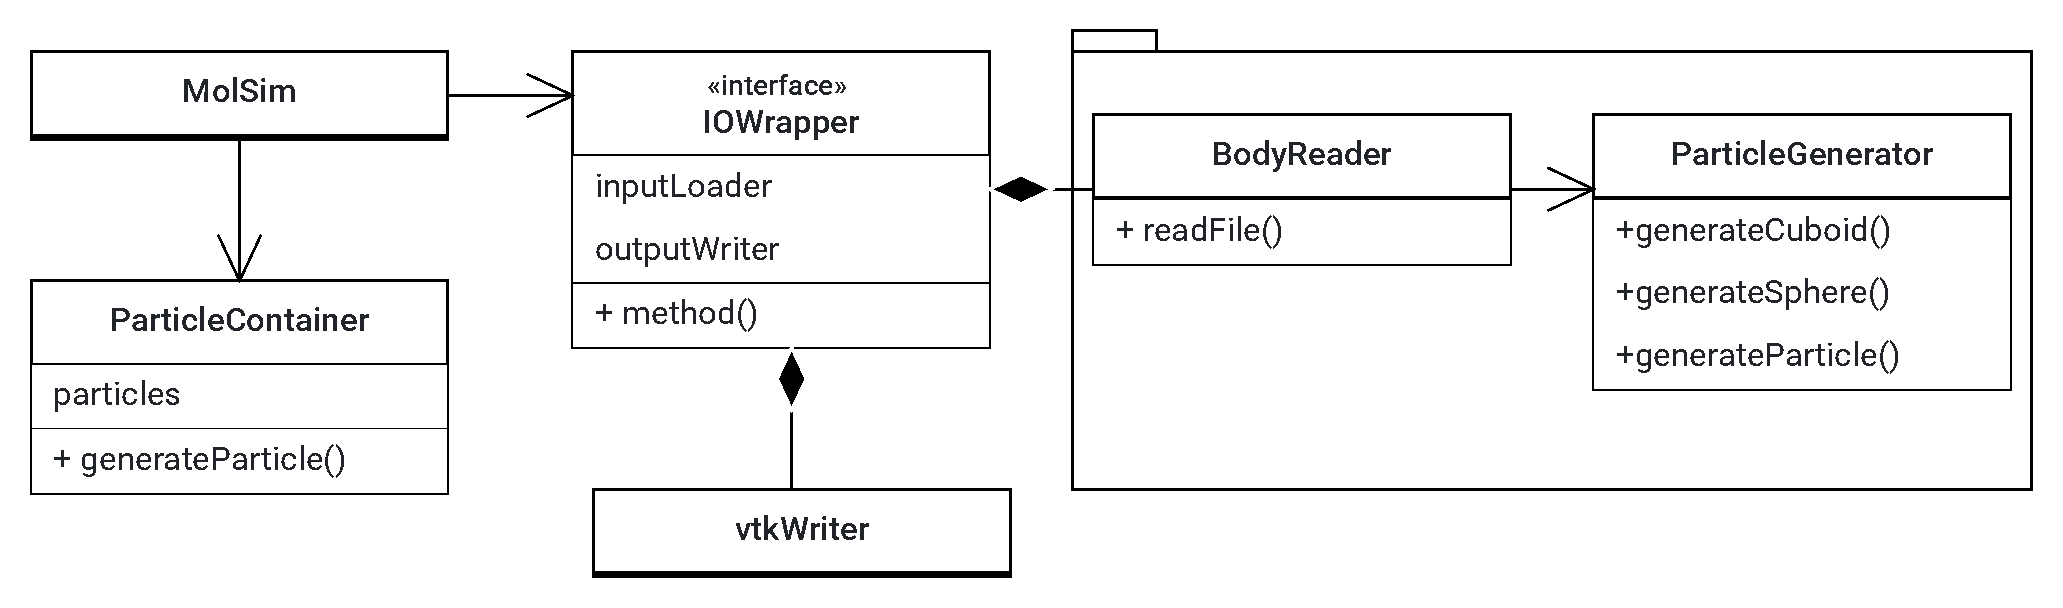
\includegraphics[width=0.7\linewidth]{IOWrapper}
		\label{fig:iowrapper}
	\end{figure}
	\large
	\centering
	input Loader gets chosen at compile time
	%\begin{itemize}
	%\item inputLoader gets chosen at compile time
	%\end{itemize}
\end{frame}


\begin{frame}[fragile]
\frametitle{Input parsing - Definition of Body}
\vspace{0.7cm}

\begin{lstlisting}[language=C++]
enum Shape {cuboid, sphere};

struct Body {
	Shape shape;   
	Eigen::Vector3d fixpoint; 
	Eigen::Vector3d dimensions; 
	double distance;
	double mass;
	Eigen::Vector3d start_velocity;
} ;
\end{lstlisting}
\end{frame}

\begin{frame}[fragile]
	\frametitle{Performance optimization}
	\large
	Force calculation is the only part relevant to performance
	\begin{lstlisting}[language=C++]
    void calculateFLennardJones() {
	//set all current forces on all particles to 0
	particleContainer.forAllParticles([](Particle &p) {
		p.setOldF(p.getF());
		p.setF({0., 0., 0.});
	});
	
	particleContainer.forAllPairs([](Particle &p1, Particle &p2){
		calculate force 
		
		p1.add_to_F(force);
		p2.add_to_F(-force);
	});
}

	\end{lstlisting}

\end{frame}

\begin{frame}
	\frametitle{Performance optimization - "Gaussian multithreading"}
	\large
	Idea: Force calculation can be multithreaded quite easily \\
	Evenly distribute Particle-pairs among multiple threads
	 
	
\end{frame}

\begin{frame}
	\frametitle{Roadblocker}
	\Large
	Spontaneously imploding Laptops and the lessons they teach us
	\large
	\begin{itemize}
		\item<1-> Get yourself familiar with alternative options available to not completely disrupt your workflow
		\item<2-> Create backups!
		\item<3-> People are nice, ask for help!
	\end{itemize}
	
\end{frame}

\begin{frame}
	\frametitle{Roadblocker}
	\Large
	Spontaneously imploding Laptops and the lessons they teach us
	\large
	\begin{itemize}
		\item Get yourself familiar with alternative options available to not completely disrupt your workflow
		\item Create backups!
		\item People are nice, ask for help!
	\end{itemize}

	\Large
	Other Roadblocker
	\large
	\begin{itemize}
		\item<1->  Missing overview over the already existing functionality and helper functions
		\item<2->  Missing communication on interfaces, project structure, etc.
	\end{itemize}
	
\end{frame}

%\frame[label=blah]{
%	\begin{center}%
%		\href{run:/usr/local/bin/mplayer -fs standard-benchmark.mp4}{
%		\includegraphics[scale=0.25]
%		{Assignment2_Presentation.pdf}}

%		\includemovie{.85\textheight}{.85\textheight}{standard-benchmark.mp4}%
%	\end{center}%
%	\note{%
%		\begin{itemize}
%			\item blah
%			\item blah
%		\end{itemize}
%	}%
%}


%%%%%%%%%%%%%%%%%%%%%%%%%%%%%%%%%%%%%%%%%%%%%%%%%%%%%
%% Folie: Gültigkeit der Masterfolien              %%
%%%%%%%%%%%%%%%%%%%%%%%%%%%%%%%%%%%%%%%%%%%%%%%%%%%%%
